\documentclass[12pt, a4paper, oneside]{ctexbook}
\usepackage{amsmath, amsthm, amssymb, bm, float,graphicx, geometry,hyperref, mathrsfs}
\geometry{left = 2.54cm, right = 2.54cm, top = 3.18cm, bottom = 3.18cm}

\title{{\Huge{\textbf{数学建模课程笔记}}}}
\author{yangmei}
\date{\today}
\linespread{1.5}
\newtheorem{theorem}{定理}[section]
\newtheorem{definition}[theorem]{定义}
\newtheorem{lemma}[theorem]{引理}
\newtheorem{corollary}[theorem]{推论}
\newtheorem{example}[theorem]{例}
\newtheorem{proposition}[theorem]{命题}

\begin{document}

\maketitle

%\pagenumbering{roman}
%\setcounter{page}{1}

%\begin{center}
%    \Huge\textbf{前言}
%\end{center}~\

%这是笔记的前言部分. 
%~\\


\newpage
\pagenumbering{Roman}
\setcounter{page}{1}
\tableofcontents
\newpage
\setcounter{page}{1}
\pagenumbering{arabic}
 
\chapter{Secret Sharing}
\section{秘密共享}

Secret Sharing: 将秘密分成若干份,分发给不同的用户。用户特定子集共同提供各自的份额,才能重构初始秘密。

Treshold Scheme$(t,n)$ :在 $n$ 人之间共享秘密,其中任意 $t\le n$ 个人可求出秘密,任意 $t-1$ 个人无法求出秘密。
\section{Combinatorial Mathematics}
问题:
Eleven scientists are working on a secret project. They wish to lock up the documents in a cabinet so that the cabinet can be opened if and only if six or more of the scientists are present. What is the smallest number of locks needed? What is the smallest number of keys to the locks each scientist must carry?

采用组合数学的方法:
“少数”与“多数”:
\begin{enumerate}
    \item 设相关人共有 $2n+1$ 个,任意 $n$ 人组成的“少数”团体不能打开安全门,任意 $n+1$ 人组成的“多数”团体可以打开安全门  
    \item 两个不同的“少数”团体联合必包含某个多数团体  
    \item 任一“少数”团体和不属该团体的任一人联合可成为多数团体        
\end{enumerate}
锁与钥匙:
\begin{enumerate}
    \item 安全门上至少需要$\binom{2n+1}n$ 把锁 $\binom{11}5=462$
    \subitem 任一“少数”团体至少有一把锁不能打开
    \subitem 任意两个 少数"各不相同
    \item 每个人至少需要$\binom{2n}n$把钥匙 $\binom{10}5 = 252$
    每个人需拥有他所不属于的所有少数" 团体所打不开的锁的钥匙 
\end{enumerate}

用数学上集合的语言来表述: 给锁编号$1,2,\cdots,l$, 打开所有门的钥匙的全集即为 $K = {1,2,\cdots,l}$,任意第$i$人拥有的钥匙集合为$S_i$,则满足:

(1) $S_{i_1} \cup S_{i_2}\cup \cdots\cup S_{i_n} \subset K/k_i$\par
(2) $S_{i_1} \cup S_{i_2}\cup \cdots \cup S_{i_n}\cup S_{i_{n+1}} = K$
 
则有:
\begin{enumerate}
    \item 那么对于不同的 $n$ 的并,所对应的 $k_i$ 不同,任意一个 $k_i$ 必有一族 $\{i_1,i_2,\cdots i_n\}$ 与之对应 则 $k_i\in K$ 共有 $C_{2n+1}^n$ 个
    \item $k_i \in S_{i_{n+1}}$,这样的 $k_i$ 有 $C_{2n+1}^{n+1}$ 个
\end{enumerate} 



\section{Shamir's Threshold Scheme}

\subsection{Lagrange Polynomial interpolation} 

\begin{theorem}
Given $k$ points in the 2-dimensional plane $(x_1 y_1) \cdots (x_k, y_k)$. 
with distinct $x_i$'s , there is one and only one polynomial $q(x)$ of degree $k - 1$ such that $q(x_i) =y_i$ for all $x_i$.        
\end{theorem}

设多项式 $q(x) = a_0 + a_1 x + a_2 x^2 + \cdots+ a_{k-1} x^{k-1}, deg(q) = k-1$,  利用$k-1$组值求得$q(x)$的各项系数  
系数矩阵:

$$\begin{vmatrix}
1 & x_1 & x_1^2 & \cdots & x_1^{k-1} \\
1 & x_2 & x_2^2 & \cdots & x_2^{k-1} \\
\vdots & \vdots & \vdots & \ddots & \vdots \\
1 & x_k & x_k^2 & \cdots & x_k^{k-1} \\
\end{vmatrix} \neq 0$$

这是一个Vandermode行列式 

\subsection{Shamir 门限机制 $(t,n)$}

任选 $t-1$ 个整数 $x_1,x_2,\cdots,x_{t-1}$ 和 n 个互不相同的整数 $c_1,c_2,\cdots,c_n$ 。
素数 $p>n+1$求 $b_j\equiv(K+c_jx_1+c_j^2x_2+\cdots+c_j^{t-1}x_{t-1})\left({\mathrm{mod}}p\right),j=1,\cdots,n$ 其
中 $K\in\mathbb{Z}$ 为秘密

$$f(c)=K+x_1c+x_2c^2+\cdots+x_{t-1}c^{t-1},b_j\equiv f(c_j)({\mathrm{mod}}p),j=1,\cdots,n$$

将秘密份额$\left(c_j,b_j\right)$告知第 $_j$ 人

\begin{proof}{证明Shamir 门限机制的合理性}
 
    (1)若 $t$ 个人 $j_1,\cdots,j_t$ 共享秘密份额 $(c_{j_i},b_{j_i}),i=1,\cdots,t$\\
    方程组 $b_i\equiv\left(K+c_{j_i}x_1+c_{j_i}^2x_2+\cdots+c_{j_i}^{t-1}x_{t-1}\right)\left({\mathrm{mod}}p\right),i=1,\cdots,t$ 在模 $p$ 意义下有唯一解
    由于系数矩阵为
    $$\begin{vmatrix}1&c_1&c_1^2&\cdots&c_1^{t-1}\\1&c_2&c_2^2&\cdots&c_2^{t-1}\\\vdots&\vdots&\vdots&\vdots&\vdots\\1&c_{t-1}&c_{t-1}^2&\cdots&c_{t-1}^{t-1}\\1&c_t&c_t^2&\cdots&c_t^{t-1}\end{vmatrix}\neq 0$$
    其行列式为Vandermode行列式,即$det = \prod_{i = 1}^{k-1} (c_i-c_{i+1})$,因此$det \neq 0$同时$rank(row) = rank(column)$,方程有唯一解。

    (2)若 $t-1$ 个人 $j_1,\cdots,j_{t-1}$共享秘密份额 $(c_{j_i},b_{j_i}),i=1,\cdots,t-1$\\
    方程组 $b_{j_i}\equiv(K+c_{j_i}x_1+c_{j_j}^2x_2+\cdots+c_{j_i}^{t-1}x_{t-1})({\mathrm{mod}}p),i=1,\cdots,t-1$ 
    N
    含 $t-1$ 个方程,$t$ 个未知数,在模 $p$ 意义下有无穷多组解
    
\end{proof}
\section{Asmuth-Bloom's Threshold Scheme}
\subsection{中国剩余定理}
\begin{definition}[逆]
    设 $a,b$ 为整数,$m$ 为正整数,若 $ab\equiv 1(\mod m)$,则称 $a$ 模 $m$ 可逆,且 $b$ 是 $a$ 在模 $m$ 意义下的逆元,记为 $a^{-1}(mod m)$    
\end{definition}
$a$对模$m$可逆的$\Leftrightarrow (a,m) = 1$,即$a$与$m$互质

\begin{example}[大衍求一术求逆元]

    \begin{figure}[H]
        \centering
        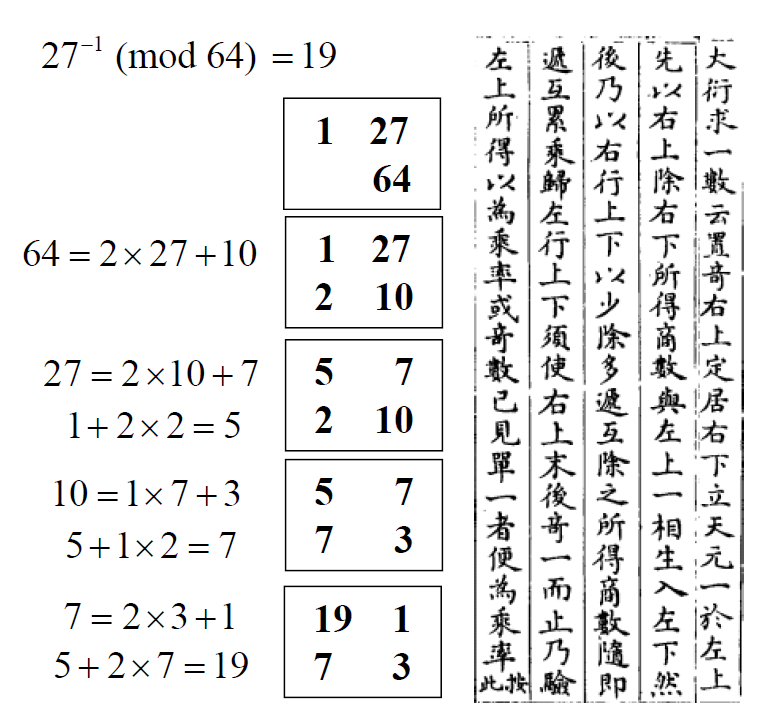
\includegraphics[width=8cm]{assets/大衍求一术.png}
    \end{figure}

\end{example}
\begin{definition}[一次同余方程]
    形如 $ax\equiv b(\mod m)$ 的方程,其中 $a,b,m$ 为整数,$m>0$。
\end{definition}

\begin{theorem}[线性同余方程有解和唯一]    
(1) 当且仅当 $gcd(a,m)|b$ 时,线性同余方程有解。\\
(2)当 $gcd(a,m)=1$ 时,方程的解为 $a^{-1}b$,且小于 $m$的非负整数解唯一。\\
其中 $a^{-1}$ 是 $a$ 在模 $m$ 意义下的逆元。      
\end{theorem}

\begin{theorem}[中国剩余定理(数论)]
    设 $m_1,m_2,\cdots,m_k$ 为两两互质的正整数,$a_1,a_2,\cdots,a_k$ 为任意整数,记$M = m_1m_2\cdots m_k$,则一次同余方程组

    $$
    \begin{cases}
    x\equiv a_1(\mod m_1)\\
    x\equiv a_2(\mod m_2)\\
    \vdots\\
    x\equiv a_k(\mod m_k)\\
    \end{cases}
    $$

    (1)有小于 $M$ 的唯一正整数解$x=M_1M_1^{-1}a_1+M_2M_2^{-1}a_2+\cdots+M_kM_k^{-1}a_k(\mod M)$,其中$M_i=M/m_i$,$M_i^{-1}$是$M_i$在模$m_i$意义下的逆元。 
    
    (2)对任意 $l\in\mathbb{Z}$,$x+l\cdot m$也是同余方程组的解.
\end{theorem}
\begin{theorem}[中国剩余定理(代数多项式)]
    设 ${f_i(x)|i = 1,\cdot,n}$ 是两两互素的多项式, $a_1(x), a_2(x),\cdots,a_n(x)$ 是 $n$ 个多项式,则存在多项式 $g(x)$,$q_i(x)(i= 1,2\cdots, n)$,使得 $g(x) = f_i(x)q_i(x) + a_i(x)$ 对一切 $i$ 成立。   
\end{theorem}

\begin{example}[物不知数]
    $$
    \begin{cases}
    &x\equiv2(\mathrm{mod}3)\quad N_1=5\cdot7=35\quad N_1^{-1}(\mathrm{mod}3)=2\\
    &x\equiv3(\mathrm{mod}5)\quad N_2=3\cdot7=21\quad N_2^{-1}(\mathrm{mod}5)=1\\
    &x\equiv2(\mathrm{mod}7)\quad N_3=3\cdot5=15\quad N_3^{-1}(\mathrm{mod}7)=1
    \end{cases}
    $$
    $$\begin{aligned}m=3\cdot5\cdot7=105&\quad35\cdot2\cdot2+21\cdot1\cdot3+15\cdot1\cdot2=233\\&\quad x=23\equiv233\mathrm{~(mod~}105)\end{aligned}$$
\end{example}  

\subsection{Asmuth-Bloom门限机制 $(t,n)$}

设秘密为 $K$\\
(1)选取整数 $p$ 与 $m_1,\cdots,m_n$\\
$p>K$ 且 $p$ 与 $m_j,1\leq j\leq n$ 互素,$m_1<\cdots<m_n$ 且 $m_1,\cdots,m_n$ 两两互素 \\
$$\frac{m_1\cdots m_t}{m_{n-t+2}\cdots m_n}>p$$
即为$m_1,\cdots,m_n$ 中任意 $t$ 个数的乘积与任意 $t-1$ 个数的乘积之比大于$p$\\
(2)令 $K^{\prime}=K+r\cdot p$,其中 $r\in\mathbb{N}$ 满足\par
(i)$0\leq r\leq\frac{m_1\cdots m_t}p-1$\par
(ii)$K^{\prime}=K+r\cdot p\leq K+m_1\cdots m_t-p<m_1\cdots m_t$\\
再令$k_j\equiv K^{\prime}({\mathrm{mod}}m_j),1\leq j\leq n$, 将秘密份额$(k_j,m_j)$告知第 $j$ 人

\begin{proof}{证明Asmuth-Bloom门限机制的合理性}\\
    $k_j\equiv K'({\mathrm{mod}}m_j),1\leq j\leq n$ ,因此$K'$满足的方程: $K'\equiv k_j({\mathrm{mod}}m_j),1\leq j\leq n$\\
    $K'=K+r\cdot p<m_1\cdots m_t$ ,$K'$对$p$取模求出$K$: $K\equiv K'(\text{mod }p)$\\
    一次同余方程组 (I) $x\equiv k_j\left({\mathrm{mod}}m_j\right),1\leq j\leq n$ 有唯一的小于 $m_1\cdots m_n$ 的非负整数解 $K'$\par
    (1)若 $t$ 个人 $j_1,\cdots,j_t$ 共享秘密份额 $\left(k_{j_i},m_{j_i}\right),i=1,\cdots,t$\\
    一次同余方程组 (II) $x\equiv k_{j_i}({\mathrm{mod}}m_{j_i}),\:i=1,\cdots,t$ 有唯一的小于 $m_{j_1}\cdots m_{j_t}$ 的正整数解 $X$\\
    $K'$也为方程(II) 的解,且 $K^{\prime}<m_1\cdots m_t<m_{j_1}\cdots m_{j_t}$ 。由中国剩余定理,解的唯一性有 $K'= X$ 
    \begin{figure}[H]
        \centering
        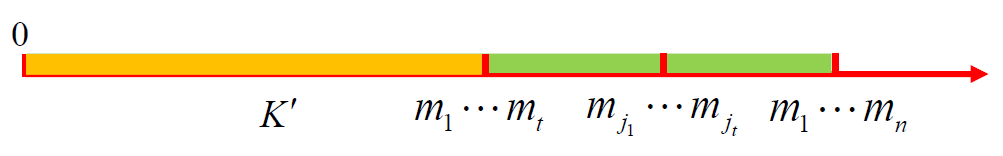
\includegraphics[width=8cm]{assets/方程ⅡK'值所在区间.png}
    \end{figure}
    (2) 若 $t-1$ 个人 $j_1,\cdots,j_{t-1}$ 共享秘密份额$\left(k_{j_i},m_{j_i}\right),i=1,\cdots,t-1$\\
    一次同余方程组 (III) $x\equiv k_{j_i}({\mathrm{mod}}m_{j_i}),\:i=1,\cdots,t-1$ 有唯一的小于$m_{j_1}\cdots m_{j_{t-1}}$的正整数解$Y$\\
    $Y+l\cdot m_{j_1}\cdots m_{j_{t-1}} < \frac{1+l}{p}*m_{j_1}m_{j_2}\cdots m_{j_{t}},l\in\mathbb{Z}$ 均为方程组 (III) 的解,  $K'$ 为这些解中的某一个, $K'$ 的限制条件仅有 $K' < m_1 m_2\cdots m_t$,因此 $K'$ 不能唯一确定 
    \begin{figure}[H]
        \centering
        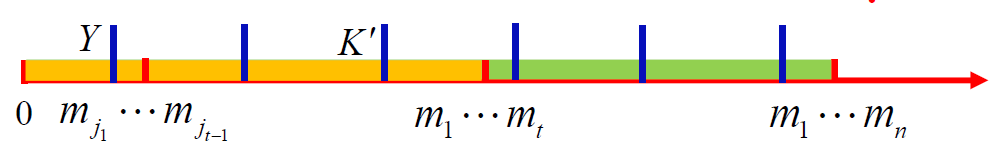
\includegraphics[width=8cm]{assets/方程ⅢK'值所在区间.png}
    \end{figure}
\end{proof}

\noindent(1)Liu, C.L. Introduction to Combinatorial Mathematics. McGraw-Hill,1968\\
(2) Shamir A. How to share a secret. Communications of the ACM, 1979, 22(11): 612-613.\\
(3) Asmuth AC, Bloom J. A modular approach to key safeguarding. IEEE Transactions on Information Theory, 29, 208-210, 1983.\\

\newpage
\chapter{Page Rank}
\section{网页重要度}
\noindent\textbf{网页重要度的原则与假设}\\
某网页重要,是因为有重要的网页链接到它,对任一网页A,确定一数值为其重要度,作为网页排序的依据
链接到网页A的所有网页对网页A的重要度均有贡献,贡献大小与这些网页自身的重要度有关
\begin{enumerate}	
    \item (传递性)重要度大的网页链接到网页A时对网页A的重要度的贡献比重要度小的网页链接到网页A时对网页A的重要度的贡献大:某网页对其它网页重要度的贡献之和等于它的重要度
    \item (等效性)网页对它所链接的每个网页的重要度的贡献相等:某网页对其它网页的重要度贡献与它所链接的网页数量呈反比
    \item (叠加性)链接到网页A的网页越多,网页A越重要:网页A的重要度是所有链接到A的网页对网页A的重要度的贡献之和
    \item (无关性)网页链接其它网页的多少,与其本身的重要度无关
\end{enumerate}	
\noindent\textbf{网页链接图}
\begin{definition}[网页链接图]
    互联网中网页之间的链接关系可用图表示,称为网络链接图。
    \begin{enumerate}
        \item[顶点]网页 $\nu_1,\nu_2,\cdots,\nu_n$ 
        \item[弧]网页间的链接关系,即若网页$\nu_i$上有链接指向网页$\nu_j$,则网络链接图中有一条以$\nu_i$为起点,$\nu_j$ 为终点的弧
        \item[出度]以某顶点为起点的弧的总数,即该网页链接的网页数量
    \end{enumerate}    
\end{definition}
\noindent\textbf{网页重要度的矩阵表示}\\
网页 $\nu_i$ 的重要度记为 $x_i$ 出度记为$q_i$
\begin{enumerate}
    \item[传递性]网页 $\nu_i$ 对其它网页重要度贡献之和为 $x_i$
    \item[等效性]网页 $\nu_i$ 对它链接的$q_i$ 个网页中的任一个的重要度贡献为$\frac{x_i}{q_i}$
    \item[叠加性]若链接到网页$\nu_j$的网页有$\nu_{j_1},\nu_{j_2},\cdots,\nu_{j_k}$,则
        $$x_j=\frac{x_{j_1}}{q_{j_1}}+\frac{x_{j_2}}{q_{j_2}}+\cdots+\frac{x_{j_k}}{q_{j_k}}$$
\end{enumerate} 

\noindent 记$p_{ij}$为网页$v_i$到$v_j$的链接概率,即$v_i$链接到$v_j$的概率,有
$$p_{ij}=\begin{cases}
\frac{1}{q_j},&\text{若}v_j\text{链接到}v_i\\
0,&\text{若}v_j\text{不链接到}v_i
\end{cases}$$
所以,上式改写为
$$x_i=\sum_{j=1}^np_{ij}x_j$$
记矩阵$\mathbf{P}=(p_{ij})_{n\times n}$为初始链接矩阵(网页$v_j$的出度列向量$\mathbf{p_j} = (p_{1j},p_{2j,\cdots,p_{nj}})^T$,$\mathbf{x}=(x_1,x_2,\cdots,x_n)^T$为网页重要度向量,
则$\mathbf{x}$为线性方程方程$\mathbf{x}=\mathbf{P}\mathbf{x}$的解。
\begin{equation}
    \mathbf{x}=\mathbf{P}\mathbf{x}
\end{equation}
\noindent(1)$\mathbf{x}$是$\mathbf{P}$的特征向量,对应的特征值为1。\\
(2)$\text{Rank}(\mathbf{I}-\mathbf{P})<n$ 由于$\mathbf{1}^T(\mathbf{I}-\mathbf{P}) = \mathbf{0}$(即说明其行向量线性相关)\\
(3)方程(2.1)一定有非零解吗,即重要度向量$\mathbf{x}$一定存在吗,这个问题之后分析。
\begin{example}[链接矩阵与重要度向量的求解]
    \begin{figure}[H]
        \centering
        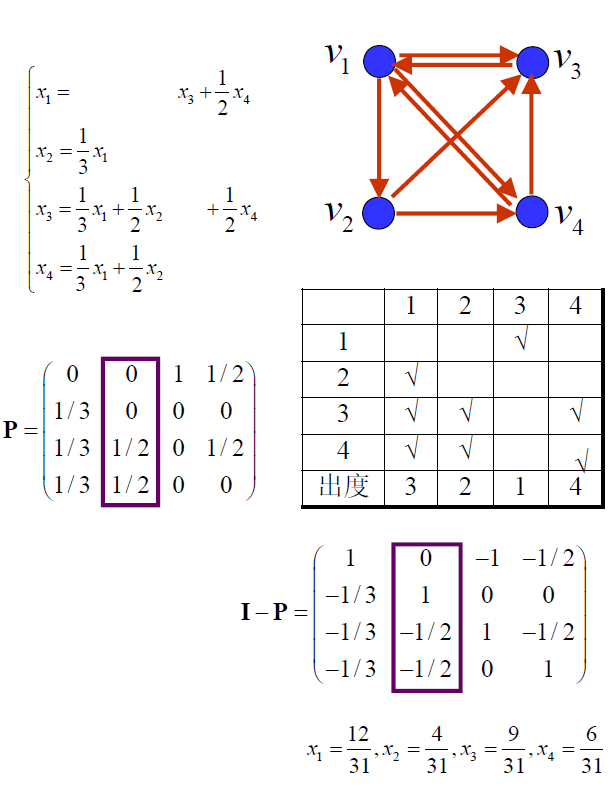
\includegraphics[width=8cm]{assets/网页重要度例题.png}
    \end{figure}
\end{example}
\section{随机矩阵}
\begin{definition}
\noindent 各行 (列) 元素之和均为 1 的非负方阵称为行 (列) 随机矩阵 (row(column) stochastic matrix)\\
各行与各列元素之和均为 1 的非负方阵称为双随机矩阵 ( doubly stochastic matrix )
\end{definition}
\begin{theorem}[随机矩阵的模最大特征值]
    任一随机矩阵的模最大特征值为 1   
\end{theorem}
\begin{proof}
    设 $\lambda$ 是行随机矩阵 $\mathbf{P}=(p_{ij})_{n\times n}$ 的特征值,非零向量 $\mathbf{X} = ( x_1, \cdots , x_n) ^{\mathrm{T} }$ 为属于特征值 $\lambda$ 的特征向量。设$|x_i|=\max_{1\leq j\leq n}|x_j|>0$\\
    由 $\mathbf{PX}=\lambda\mathbf{X}$,可得 $\lambda x_i=\sum_{j=1}^np_{ij}x_j$。 两边取模,$|\lambda\|x_i|=|\lambda x_i|=\left|\sum_{i=1}^np_{ij}.x_j\right|\leq\sum_{i=1}^n|p_{ij}\|x_j|\leq|x_i|\sum_{i=1}^n|p_{ij}|=|x_i|$, 即$|\lambda|\leq1$
\end{proof}
\section{链接矩阵}
\noindent\textbf{链接矩阵的基本性质}\\
(1)链接矩阵 $\mathbf{P}$ 的每列元素之和为 1 ,为列随机矩阵\\
(2)初始链接矩阵和修正链接矩阵$\mathbf{P}$一定具有特征值为$1$的非零特征向量\\
(3)  $\mathbf{1}^T \mathbf{P} = \mathbf{1}^T$
\subsection{悬挂网页修正}

\end{document} 